\documentclass{beamer}
% Required packages
\usepackage{amsmath}
\usepackage{physics}
\usepackage{graphicx}
\usepackage{siunitx}
\usepackage{xcolor}
\usepackage{tikz}
% Set image search paths
\graphicspath{{../images/}{../../shared/images/}}

% Define custom colors for DS9 theme
\definecolor{ds9blue}{RGB}{25,25,112}
\definecolor{ds9gold}{RGB}{218,165,32}
\definecolor{ds9grey}{RGB}{105,105,105}
\definecolor{ds9red}{RGB}{178,34,34}
% Set up the Madrid theme with custom colors
\usetheme{Madrid}
\usecolortheme{whale}
\setbeamercolor{palette primary}{bg=ds9blue,fg=white}
\setbeamercolor{palette secondary}{bg=ds9grey,fg=white}
\setbeamercolor{palette tertiary}{bg=ds9gold,fg=black}
\setbeamercolor{palette quaternary}{bg=ds9red,fg=white}
\setbeamercolor{structure}{fg=ds9blue}
\setbeamercolor{title}{fg=ds9gold}
\setbeamercolor{subtitle}{fg=ds9gold}
\setbeamercolor{frametitle}{bg=ds9blue,fg=white}
\setbeamercolor{block title}{bg=ds9blue,fg=white}
\setbeamercolor{block body}{bg=ds9grey!20,fg=black}

% Title page configuration
\title{Lesson CH:4}
\subtitle{Newton's Laws of Motion}
\author{Mr. Gullo}
\date{September 2024}

% Add logo
\logo{
\includegraphics[width=0.1\linewidth]{phys12-shared-cinec-logo.png}}


% Table of contents at the beginning of each section
\AtBeginSection[]
{
  \begin{frame}
    \frametitle{Table of Contents}
    \tableofcontents[currentsection]
  \end{frame}
}

\begin{document}

\frame{\titlepage}

\section{Overview}

\begin{frame}
\frametitle{Newton's Three Laws of Motion}

\begin{itemize}
    \item \textbf{First Law: The Law of Inertia}
    \begin{equation*}
    \sum \vec{F} = \vec{0} \Rightarrow \vec{v} = \text{constant}
    \end{equation*}
    If no net force, velocity remains constant (including zero).

    \item \textbf{Second Law: Force, Mass, and Acceleration}
    \begin{equation*}
    \vec{F} = m\vec{a} \quad \text{or} \quad \vec{a} = \frac{\vec{F}}{m}
    \end{equation*}
    Net force equals mass times acceleration.

    \item \textbf{Third Law: Action and Reaction}
    \begin{equation*}
    \vec{F}_{A \text{ on } B} = -\vec{F}_{B \text{ on } A}
    \end{equation*}
    Forces between objects are equal and opposite.
\end{itemize}

\vspace{0.5cm}
\small{Note: $\vec{F}$ is force, $m$ is mass, $\vec{a}$ is acceleration, $\vec{v}$ is velocity.}
\end{frame}

\begin{frame}
\frametitle{Newton's Second Law in Detail}
\begin{itemize}
    \item Acceleration ($\vec{a}$) is defined as a change in velocity, either in magnitude or direction, or both.
    \item Newton's second law of motion states that the acceleration of a system is directly proportional to and in the same direction as the net external force acting on the system, and inversely proportional to its mass.
    \item In equation form:
    \[\vec{a}=\frac{\vec{F}_{\text{net}}}{m}\]
    \item Often written in the more familiar form:
    \[\vec{F}_{\text{net}}=m\vec{a}\]
    \item $\vec{F}_{\text{net}}$ represents the net external force acting on the system.
    \item $m$ is the mass of the system.
\end{itemize}
\end{frame}

\begin{frame}
\frametitle{Weight and Free Fall}
\begin{itemize}
    \item Weight ($\vec{w}$) is defined as the force of gravity acting on an object of mass $m$.
    \item The object experiences an acceleration due to gravity $\vec{g}$:
    \[\vec{w}=m\vec{g}\]
    \item If the only force acting on an object is due to gravity, the object is in free fall.
    \item On Earth, the acceleration due to gravity is approximately 9.8 m/s² downward.
\end{itemize}
\end{frame}

\begin{frame}
\frametitle{Forces on an Inclined Plane}
When objects rest on an inclined plane that makes an angle $\theta$ with the horizontal surface:
\begin{itemize}
    \item The weight of the object can be resolved into components that act perpendicular ($\vec{w}_{\perp}$) and parallel ($\vec{w}_{\|}$) to the surface of the plane.
    \item These components can be calculated using:
    \begin{align*}
    w_{\|} &= |\vec{w}| \sin(\theta) = mg \sin(\theta) \\
    w_{\perp} &= |\vec{w}| \cos(\theta) = mg \cos(\theta)
    \end{align*}
    \item $\vec{w}_{\|}$ is the component causing the object to slide down the plane.
    \item $\vec{w}_{\perp}$ is the component balanced by the normal force from the plane.
\end{itemize}
\end{frame}

\begin{frame}
\begin{figure}
    \centering
    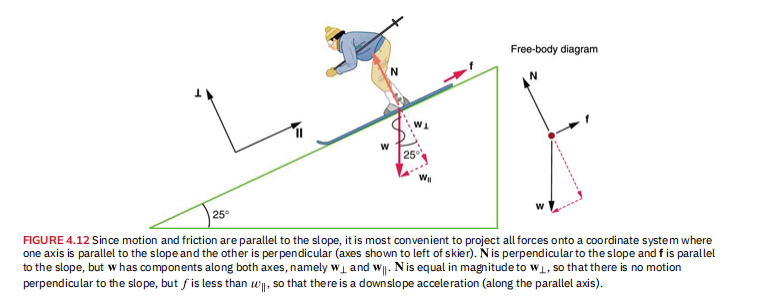
\includegraphics[width=1.0\linewidth]{CH4/Screenshot 2024-10-21 152424.png}
\end{figure}
\end{frame}
\begin{frame}
\frametitle{Tension and Normal Force}
\begin{itemize}
    \item Tension ($\vec{T}$) is the pulling force that acts along a stretched flexible connector, such as a rope or cable.
    \item When a rope supports the weight of an object at rest:
    \[|\vec{T}| = mg\]
    \item Normal force ($\vec{N}$) is the supporting force applied by a surface to an object that is at rest on the surface.
    \item On a horizontal, non-accelerating surface:
    \[|\vec{N}| = mg\]
    \item The normal force is always perpendicular to the surface.
\end{itemize}
\end{frame}

\begin{frame}
\begin{figure}
    \centering
    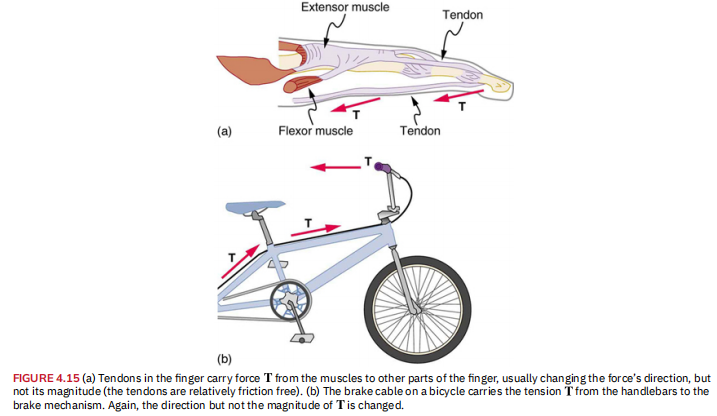
\includegraphics[width=1\linewidth]{CH4/Screenshot 2024-10-21 152741.png}
\end{figure}
\end{frame}

\begin{frame}
\frametitle{Problem-Solving Strategy}
To solve problems involving Newton's laws of motion:
\begin{enumerate}
    \item Draw a sketch of the problem.
    \item Identify known and unknown quantities, and the system of interest.
    \item Draw a free-body diagram:
    \begin{itemize}
        \item Represent the object as a dot.
        \item Draw vectors for all forces acting on the object.
        \item Resolve non-horizontal/vertical vectors into components.
    \end{itemize}
    \item Apply Newton's second law in the horizontal and vertical directions:
    \begin{itemize}
        \item If no acceleration in a direction: $F_{\text{net}} = 0$
        \item If acceleration present: $F_{\text{net}} = ma$
    \end{itemize}
    \item Solve the resulting equations.
    \item Check your answer: Is it reasonable? Are the units correct?
\end{enumerate}
\end{frame}

\begin{}

\section{4.3 NEWTON'S SECOND LAW OF MOTION: CONCEPT OF A SYSTEM}

\begin{frame}
\frametitle{Problem 4}
\begin{itemize}
    \item Since astronauts in orbit are apparently weightless, a clever method of measuring their masses is needed to monitor their mass gains or losses to adjust diets. One way to do this is to exert a known force on an astronaut and measure the acceleration produced. Suppose a net external force of 50.0 N is exerted and the astronaut's acceleration is measured to be $0.893 \mathrm{~m} / \mathrm{s}^{2}$.
    \item (a) Calculate her mass.
    \item (b) By exerting a force on the astronaut, the vehicle in which they orbit experiences an equal and opposite force. Discuss how this would affect the measurement of the astronaut's acceleration. Propose a method in which recoil of the vehicle is avoided.
\end{itemize}
\end{frame}

\begin{frame}
\frametitle{Problem 4 - Solution}
Solution:
\begin{itemize}
    \item[(a)] $m = \frac{\text{net} F}{a} = \frac{50.0 \mathrm{~N}}{0.893 \mathrm{~m} / \mathrm{s}^{2}} = 56.0 \mathrm{kg}$
    \item[(b)] $a_{\text{meas}} = a_{\text{astro}} + a_{\text{ship}}$, where: $a_{\text{ship}} = \frac{m_{\text{astro}} a_{\text{astro}}}{m_{\text{ship}}}$
    \item If the force could be exerted on the astronaut by another source (other than the spaceship), then the spaceship would not experience a recoil.
\end{itemize}
\end{frame}

\begin{frame}
\frametitle{Derivation of Ship's Acceleration}
\small
\begin{itemize}
    \item[1)] Newton's Third Law: Force on astronaut equals negative force on ship
    $$F_{\text{on astro}} = -F_{\text{on ship}}$$
    
    \item[2)] Express forces using Newton's Second Law (F = ma):
    $$m_{\text{astro}} a_{\text{astro}} = -m_{\text{ship}} a_{\text{ship}}$$
    
    \item[3)] Rearrange to isolate $a_{\text{ship}}$:
    \begin{align*}
        -m_{\text{ship}} a_{\text{ship}} &= m_{\text{astro}} a_{\text{astro}} \\
        m_{\text{ship}} a_{\text{ship}} &= -m_{\text{astro}} a_{\text{astro}} \\
        a_{\text{ship}} &= -\frac{m_{\text{astro}} a_{\text{astro}}}{m_{\text{ship}}}
    \end{align*}
    
    \item[4)] Drop negative sign for magnitude:
    $$a_{\text{ship}} = \frac{m_{\text{astro}} a_{\text{astro}}}{m_{\text{ship}}}$$
    
    \item Interpretation: Ship's acceleration is proportional to astronaut's mass and acceleration, inverse to ship's mass.
\end{itemize}
\end{frame}

\section{4.4 NEWTON'S THIRD LAW OF MOTION: SYMMETRY IN FORCES}

\begin{frame}
\frametitle{Problem 16}
A rugby player is being pushed backward by an opposing player who is exerting a force of 800 N on him. The mass of the losing player plus equipment is 90.0 kg, and he is accelerating at $1.20 \mathrm{~m} / \mathrm{s}^{2}$ backward.
\begin{itemize}
    \item[(a)] What is the force of friction between the losing player's feet and the grass?
    \item[(b)] What force does the winning player need to exert on the ground to move forward at the same acceleration if his mass plus equipment is 110 kg?
    \item[(c)] Draw a sketch of the situation showing the system of interest used to solve each part.
\end{itemize}
\end{frame}

\begin{frame}
\frametitle{Problem 16 - Part (a)}
\begin{block}{Question}
What is the force of friction between the losing player's feet and the grass?
\end{block}
\begin{block}{Knowns and Unknowns}
\textbf{Knowns:}
\begin{itemize}
    \item $F_{\text{opposing}} = 800$ N
    \item $m_{\text{losing}} = 90.0$ kg
    \item $a = 1.20$ m/s² backward
\end{itemize}
\textbf{Unknown:}
\begin{itemize}
    \item $F_{\text{friction}}$ (force of friction)
\end{itemize}
\end{block}
\begin{block}{Solution}
net $F = F - f = ma$
\begin{equation*}
f = F - ma = 800 \mathrm{~N} - (90.0 \mathrm{kg})(1.20 \mathrm{~m} / \mathrm{s}^{2}) = \underline{692 \mathrm{~N}}
\end{equation*}
\end{block}
\end{frame}

\begin{frame}
\frametitle{Problem 16 - Part (b)}
\begin{block}{Question}
What force does the winning player exert on the ground to move forward if his mass plus equipment is 110 kg?
\end{block}
\begin{block}{Knowns and Unknowns}
\textbf{Knowns:}
\begin{itemize}
    \item $m_{\text{winning}} = 110$ kg
    \item $a = 1.20$ m/s² (same as losing player, in opposite direction)
    \item $F_{\text{friction}} = 692$ N (calculated in part a)
\end{itemize}
\textbf{Unknown:}
\begin{itemize}
    \item $F_{\text{ground}}$ (force exerted on the ground)
\end{itemize}
\end{block}
\begin{block}{Solution}
\begin{equation*}
F = ma + f = (110 \mathrm{kg} + 90.0 \mathrm{kg})(1.20 \mathrm{~m} / \mathrm{s}^{2}) + 692 \mathrm{~N} = 932 \mathrm{~N}
\end{equation*}
\end{block}
\end{frame}


\begin{frame}
\frametitle{Problem 16 - Solution (c)}
\begin{itemize}
\item[(c)] Draw a sketch of the situation showing the system of interest used to solve each part.
    \item[(a)] What is the force of friction between the losing player's feet and the grass?
   
\end{itemize}
\begin{figure}
    \centering
    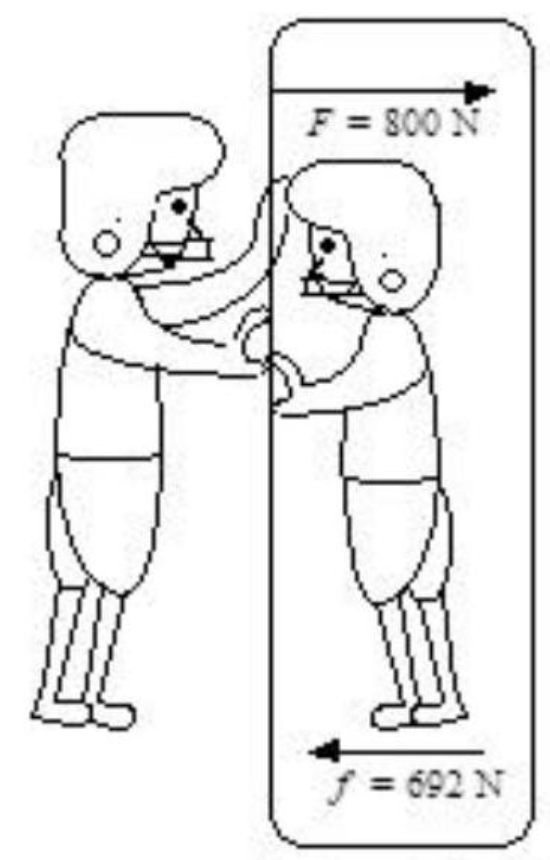
\includegraphics[width=0.25\linewidth]{CH4/Screenshot 2024-10-18 111640.png}
\end{figure}
\end{frame}

\begin{frame}
\frametitle{Problem 16 - Solution (c)}
\begin{itemize}
\item[(c)] Draw a sketch of the situation showing the system of interest used to solve each part.
   \item[(b)] What force does the winning player exert on the ground to move forward if his mass plus equipment is 110 kg?
\end{itemize}
\begin{figure}
    \centering
    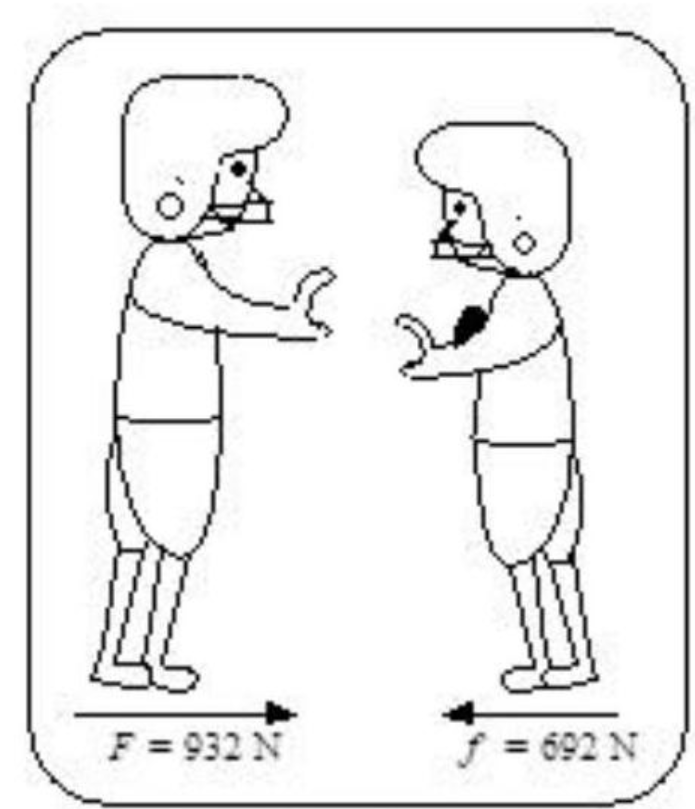
\includegraphics[width=0.25\linewidth]{CH4/Screenshot 2024-10-18 111809.png}
\end{figure}
\end{frame}

\section{4.5 Normal, Tension, and Other Examples of Forces}

\begin{frame}
\frametitle{Problem 17}
Two teams of nine members each engage in a tug of war. Each of the first team's members has an average mass of 68 kg and exerts an average force of 1350 N horizontally. Each of the second team's members has an average mass of 73 kg and exerts an average force of 1365 N horizontally.
\begin{itemize}
    \item[(a)] What is the acceleration of the two teams?
    \item[(b)] What is the tension in the section of rope between the teams?
\end{itemize}
\end{frame}


\begin{frame}
\frametitle{Problem 17 - Solution (a)}
\begin{figure}
    \centering
    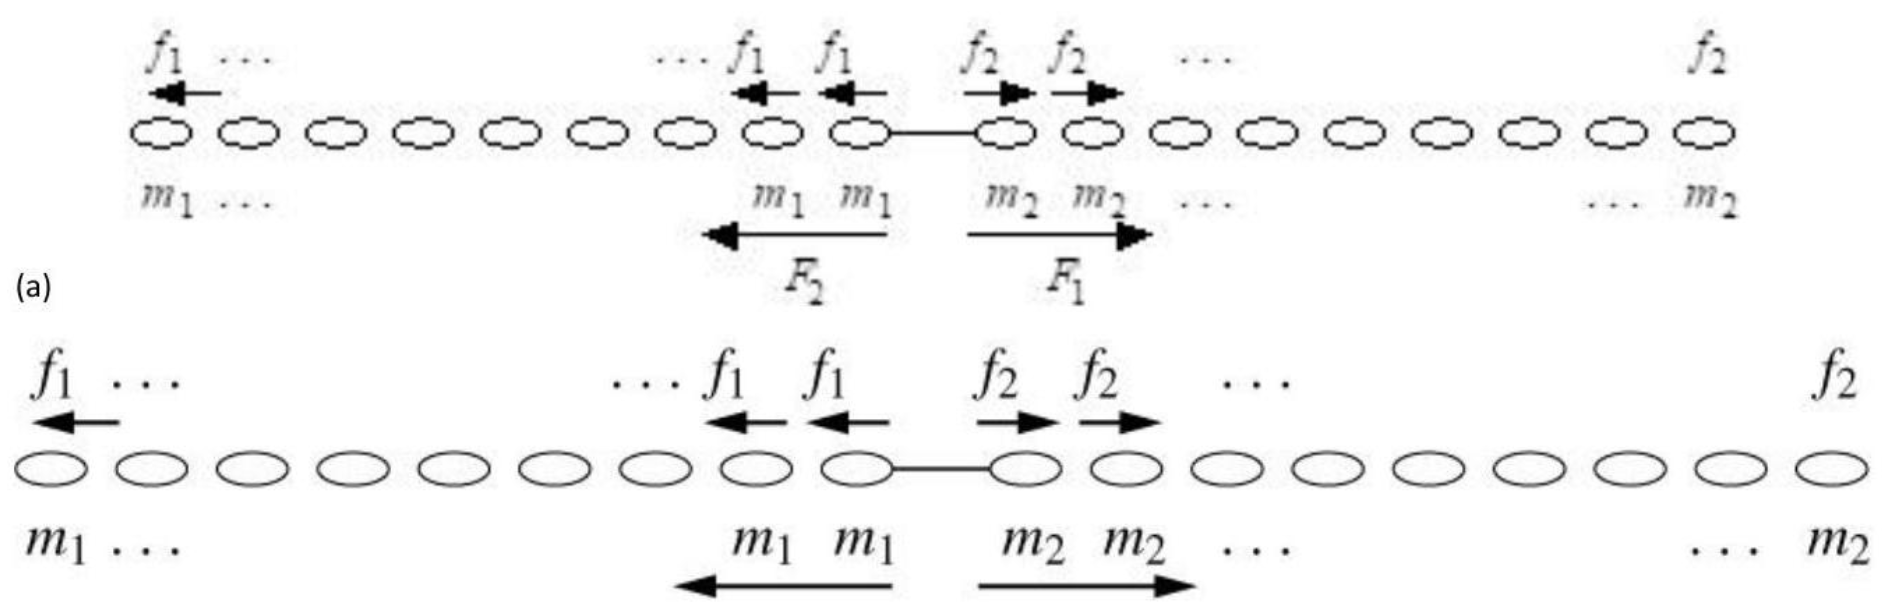
\includegraphics[width=0.7\linewidth]{CH4/Screenshot 2024-10-18 111908.png}
\end{figure}

net $F = Ma$; $f_1 = 1350 \mathrm{~N}$; $f_2 = 1365 \mathrm{~N}$

$9(f_2 - f_1) = 9(m_1 + m_2)a$; $m_1 = 68 \mathrm{~kg}$; $m_2 = 73 \mathrm{~kg}$

\begin{equation*}
a = \frac{f_2 - f_1}{m_1 + m_2} = \frac{1365 \mathrm{~N} - 1350 \mathrm{~N}}{68 \mathrm{~kg} + 73 \mathrm{~kg}} = 0.1064 \mathrm{~m} / \mathrm{s}^{2} = \underline{0.11 \mathrm{~m} / \mathrm{s}^{2}}
\end{equation*}

Thus, the heavy team wins. Note that the difference $1365 \mathrm{~N} - 1350 \mathrm{~N} = 15 \mathrm{~N}$ limits the answer to two significant figures.
\end{frame}

\begin{frame}
\frametitle{Problem 17 - Solution (b)}
\begin{itemize}
    \item[(b)] What is the tension in the section of rope between the teams?
\end{itemize}
\begin{figure}
    \centering
    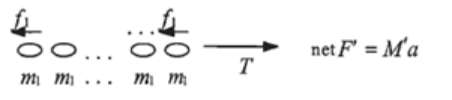
\includegraphics[width=0.5\linewidth]{CH4/Screenshot 2024-10-20 145707.png}
\end{figure}

\begin{equation*}
T - 9f_1 = 9m_1a \Rightarrow T = 9m_1a + 9f_1
\end{equation*}
\begin{equation*}
T = 9(68 \text{ kg})(0.1064 \text{ m/s}^2) + 9(1350 \text{ N}) = \underline{1.2 \times 10^{4} \text{ N}}
\end{equation*}
\end{frame}

\begin{frame}
\frametitle{Problem 17 - Explanation}
Explanation:
\begin{itemize}
    \item[(a)] We use Newton's Second Law for the entire system: $F = Ma$
    \begin{itemize}
        \item The net force is the difference between the forces of the two teams
        \item We divide by the total mass to find acceleration
    \end{itemize}
    \item[(b)] We consider the forces on one team
    \begin{itemize}
        \item Use Newton's Second Law: $T - 9f_1 = 9m_1a$
        \item Solve for $T$ and substitute known values
    \end{itemize}
    \end{itemize}
\end{frame}

\section{4.6 PROBLEM-SOLVING STRATEGIES}

\begin{frame}
\frametitle{Problem 28}
Commercial airplanes are sometimes pushed out of the passenger loading area by a tractor.
\begin{itemize}
    \item[(a)] An 1800-kg tractor exerts a force of $1.75 \times 10^{4} \text{ N}$ backward on the pavement, and the system experiences forces resisting motion that total 2400 N. If the acceleration is $0.150 \text{ m/s}^{2}$, what is the mass of the airplane?
    \item[(b)] Calculate the force exerted by the tractor on the airplane, assuming 2200 N of the friction is experienced by the airplane.
    \item[(c)] Draw two sketches showing the systems of interest used to solve each part, including the free-body diagrams for each.
\end{itemize}
\end{frame}

\begin{frame}
\frametitle{Problem 28 - Solution (a)}
\textbf{Question:} An 1800-kg tractor exerts a force of $1.75 \times 10^{4} \text{ N}$ backward on the pavement, and the system experiences forces resisting motion that total 2400 N. If the acceleration is $0.150 \text{ m/s}^{2}$, what is the mass of the airplane?

\vspace{0.5cm}

\textbf{Solution:}
net $F = Ma = (m_a + m_t)a = F - f$, so that: $m_a = \frac{F - f}{a} - m_t$
\begin{equation*}
m_a = \frac{1.75 \times 10^{4} \text{ N} - 2400 \text{ N}}{0.150 \text{ m/s}^{2}} - 1800 \text{ kg} = \underline{9.89 \times 10^{4} \text{ kg}}
\end{equation*}
\end{frame}

\begin{frame}
\frametitle{Problem 28 - Solution (b)}
\textbf{Question:} Calculate the force exerted by the tractor on the airplane, assuming 2200 N of the friction is experienced by the airplane.

\vspace{0.5cm}

\textbf{Solution:}
net $F = F' - f' = m_a a$
\begin{equation*}
F' = m_a a + f' = (9.89 \times 10^{4} \text{ kg})(0.150 \text{ m/s}^{2}) + 2200 \text{ N} = \underline{1.70 \times 10^{4} \text{ N}}
\end{equation*}
\end{frame}

\begin{frame}
\frametitle{Problem 28 - Solution (c)}
\textbf{Question:} Draw two sketches showing the systems of interest used to solve each part, including the free-body diagrams for each.

\vspace{0.5cm}

\textbf{Solution:}

\begin{figure}
    \centering
    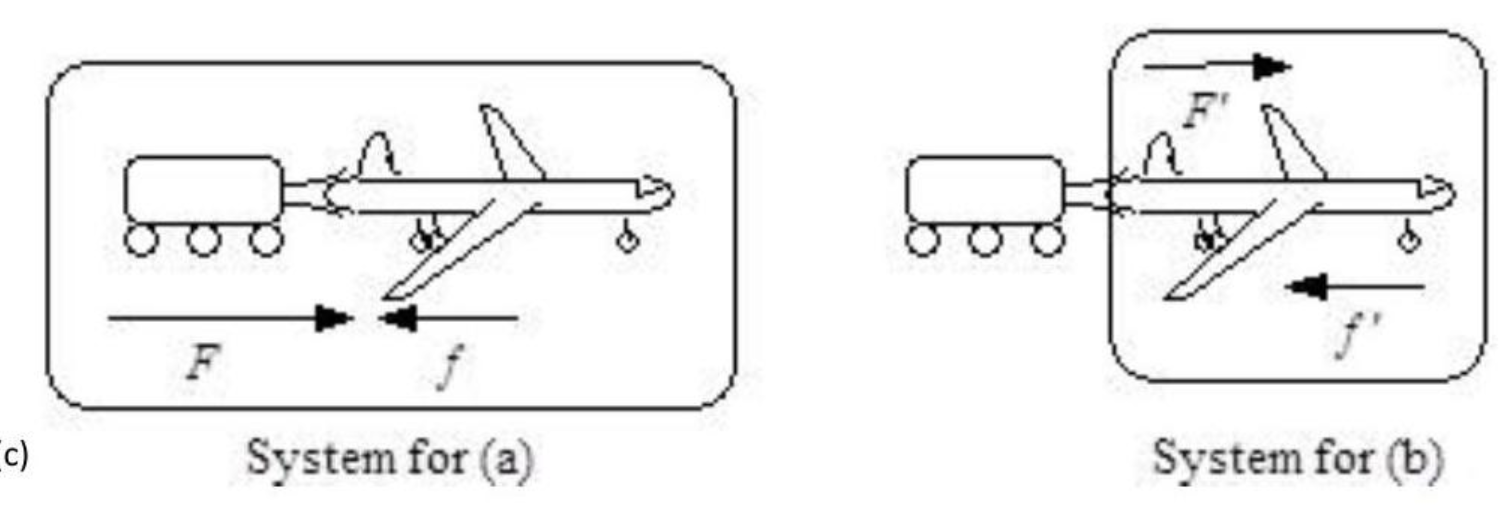
\includegraphics[width=0.5\linewidth]{CH4/Screenshot 2024-10-18 111935.png}
\end{figure}
\end{frame}

\begin{frame}
\frametitle{Problem 28 - Explanation}
Explanation:

    \item[(a)] We use Newton's Second Law for the entire system: F = Ma
    \begin{itemize}
        \item Substitute the given force, friction, and acceleration
        \item Solve for the airplane's mass
    \end{itemize}
    \item[(b)] We use Newton's Second Law for just the airplane: $F' - f' = m_\text{airplane} a$
    \begin{itemize}
        \item Solve for F' and substitute known values
    \end{itemize}
    
\end{frame}


\begin{frame}

\frametitle{Conclusion}
\begin{itemize}
\item We've explored various applications of Newton's Laws of Motion:
\begin{itemize}
\item Measuring mass in weightless environments
\item Analyzing forces in sports (rugby and tug of war)
\item Calculating forces in aircraft towing
\end{itemize}
\item Key takeaways:
\begin{itemize}
\item Newton's Second Law (F = ma) is crucial for solving these problems
\item Consider all forces acting on a system
\item Break down complex situations into simpler components
\item Pay attention to vector directions and sign conventions
\end{itemize}
\item Practice solving homework problems to reinforce your understanding of Newton's Laws
\end{itemize}
\end{frame}
\end{document}